% !TeX root = RJwrapper.tex
\title{Advancing reproducible research by publishing R markdown notebooks as
interactive sandboxes using the `learnr' package}
\author{by Chak Hau Michael Tso, Michael Hollaway, Rebecca Killick, Peter Henrys, Don Monteith, John Watkins, and Gordon Blair}

\maketitle

\abstract{%
Various R packages and best practices have played a pivotal role to
promote the FAIR principles of open science. For example, (1)
well-documented R scripts and notebooks with rich narratives are
deposited at a trusted data centre, (2) R markdown interactive notebooks
can be run on-demand as a web service, and (3) R Shiny web apps provide
nice user interfaces to explore research outputs. However, notebooks
require users to go through the entire analysis and can easily break it,
while Shiny apps do not expose the underlying code and require extra
work for UI design. We propose using the \emph{learnr} package to expose
certain code chunks in R markdown so that users can readily experiment
with them in guided, isolated and resettable code sandboxes. Our
approach does not replace the existing use of notebooks and Shiny apps,
but it adds another level of abstraction between them to promote
reproducible science.
}

\hypertarget{introduction}{%
\subsection{Introduction}\label{introduction}}

There has been considerable recognition to the need to promote open and
reproducible science in the past decade. The FAIR principles
\citep{Wilkinson2016a, Stall2019}
(\url{https://www.go-fair.org/fair-principles/}) of reproducble research
are now known to most scientists. While significant advances has been
made through the adoption of various best practices and policies
(e.g.~requirements from funders and publishers to archive data and
source code, metadata standards), there remains considerable barriers to
further advance open science and meet reproducible science needs. One of
such issues the availability of various levels of abstraction of the
same underlying analysis and code base to collaborate and engage with
different stakeholders of diverse needs \citep{Blair2019, Hollaway2020}.
For complex analysis or analysis that utilize a more advanced computing
environment, it is essential to provide the capability to allow users to
interact with the analysis at a higher level.

Existing approach to reproducible research focuses on either documenting
an entire analysis or allows user-friendly interaction. Within the R
ecosystem, R script and notebooks allow reserachers to work together and
others to view the entire workflow, while R Shiny apps \citep{shiny}
allows rapid showcase of methods and research outcomes to users with
less experience. R Shiny has been widely adopted to share research
output and engage stakeholders since its conception in 2013. A recent
review \citep{Kasprzak} shows that bioinformatics is the subject with
the most Shiny apps published in journals while earth and envrironmental
science ranks second. Shiny apps are especially helpful to create
reproducible analysis \citep[e.g.~examples in][]{Hollaway2020} and
explore different scenarios \citep[e.g.][]{Whateley2015, Mose2018}.
Finally, the interactivity of Shiny apps makes it a excellent tool for
teaching\citep[e.g.][]{Williams2017, adventr}. However, not all user
needs fit nicely into this dichotomy. Some users may only want to adopt
a small fraction of an analysis for their work, while others may simply
want to modify a few parts of the analysis in order to test alternative
hypothesis. Current use of notebooks do not seem to support such diverse
needs as notebook \emph{elements} are not easily reproducible. This
issue essentially applies to all coding languages.

One potential way to address the problem described above is to allow
users to experiment with the code in protected computing environment.
This is not limited to creating instances for users to re-run the entire
code. Rather, this can also be done by exposing specific parts of a
notebook as editable code boxes, as seen in many interactive tutorial
webpages for various coding languages. Recenty, while discussing next
steps for fostering reproducible research in artificial intelligence,
\citet{Carter2019} lists creating a protected computing environment
(`data enclave' or `sandbox') for reviewers to log in and explore as one
of the solutions. In software engineering, a sandbox is a testing
environment that isolates untested code changes and outright
experimentation from the production environment or repository, in the
context of software development including Web development and revision
control. Making a sandbox environment available for users to test and
explore various changes to the code that leads to research outputs is a
great step to further open science. Current practice of open science
largely requires users to assemble the notebooks, scripts and data files
provided in their own computing environment, which requires significant
amount of time and effort. A sandbox environment can greatly reduce such
barriers and if such sandboxes are available as a web service, users can
explore and interact with the code that generates the research outputs
at the convience of their own web browser on demand.

In this paper, we describe a rapid approach to create and publish
``sandbox'' Shiny apps from R markdown documents using the \emph{learnr}
package, with the aim to bridge the gap between typical R markdown
notebook and typical Shiny apps in terms of levels of abstraction.

\hypertarget{the-learnr-r-package}{%
\subsection{\texorpdfstring{The \emph{learnr} R
package}{The learnr R package}}\label{the-learnr-r-package}}

\emph{learnr} \citep{learnr} is an R package developed by RStudio to
rapidly create interactive tutorials. It follows the general
\emph{Rmarkdowon} (the file has .Rmd extensions) architecture and
essentially creates a pre-rendered Shiny document similar to the way
Shiny UI components can be added to any R markdown documents. To create
a \emph{learnr} tutorial, the user chooses a \emph{learnr} R markdown
template. This template is not different from other .Rmd files, except
it requires additional chunk arguments to control the sandbox
appearances. The two main feature of the \emph{learnr} package are the
``exercise'' and ``quiz'' options. The former allow users to directly
type in code, execute it, and see its results to test their knowlege
while the latter allow other question types such as multiple choice.
Both of these options include auto-graders, hints, and instructor
feedback options. Additonal overall options include setting time limits
and option to forbid users to skip sections. Like any Shiny apps,
\emph{learnr} sites can be easily embedded to other sites, as seen in
this example \citep{rmrwr}.

Although the \emph{learnr} package has existed for a few years now, it
is relatively not well known and has mostly been used for simple
tutorial apps designed for R beginners. We propose a novel application
of the \emph{learnr} package to advance reproducible research, which we
outline in the next section.

\hypertarget{approach-using-learnr-for-reproducible-research-sandboxes}{%
\subsection{\texorpdfstring{Approach: Using \emph{learnr} for
reproducible research
`sandboxes'}{Approach: Using learnr for reproducible research `sandboxes'}}\label{approach-using-learnr-for-reproducible-research-sandboxes}}

Our approach is to publish R notebooks and serve parts of the notebooks
as interactive sandboxes to allow users to re-create certain elements of
a published notebook containing research outputs. We disable the
auto-graders and any quiz-like functionality of \emph{learnr} while
keeping the sandboxes. Notebook authors can go through their notebook
and select the code chunks that they would allow users to experiment,
while the others are rendered as static code snippets.

Recognizing \emph{learnr} documents are themselves \emph{shiny} sites,
our approach essentially allows the publication of notebooks in the form
of web apps. However, unlike a typical \emph{shiny} site, they are
pre-rendered shiny documents, meaning the user do not need to prepare
seprate UI (i.e.~user interface) and Server elements. Advanced users can
modify the site appearance by supplying custom design in .css files.

Here, we first show the skeleton of a R markdown (.Rmd) file for a
\emph{learnr} document.

\begin{figure}
     \centering
     \begin{subfigure}[b]{0.2\textwidth}
         \centering
         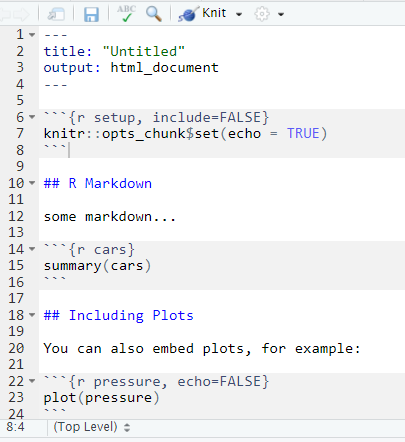
\includegraphics[width=0.2\textwidth]{skeleton-md}
         \caption{A typical .Rmd file}
     \end{subfigure}
     \hfill
     \begin{subfigure}[b]{0.2\textwidth}
         \centering
         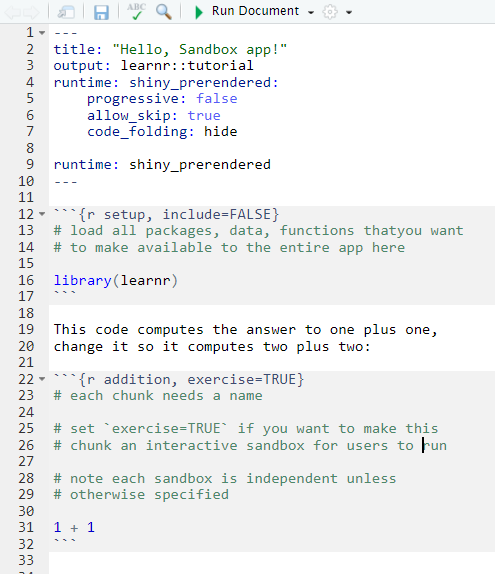
\includegraphics[width=0.2\textwidth]{skeleton}
         \caption{A sandbox app .Rmd file}
     \end{subfigure}

\caption[A comparison of minimal examples of a typical .Rmd document and a .Rmd document for an interactive sandbox app]{A comparison of minimal examples of a typical .Rmd document and a .Rmd document for an interactive sandbox app.}\label{fig:fig_skeleton}
\end{figure}


Notice that it is very similar to a typical .Rmd file where there is a
mixture of narratives written in markdown and R code chunks, in
addtional to a YAML header. However, there are a couple of important
exceptions, namely the use of the \texttt{exercise} chunk options and
different output type in the YAML header.

Next, we outline the steps an author needs to take to publish R
notebooks as interactive sandboxes:

\begin{enumerate}
\def\labelenumi{\arabic{enumi}.}
\tightlist
\item
  All research output is included in the form of a well-documented R
  markdown document
\item
  Open a new \emph{learnr} R markdown template. Copy the content of the
  original notebook
\item
  For the code chunks that you would like to become sandboxes, add
  \texttt{exercise=TRUE}. Make sure it has a unique chunk name. It may
  look something like this:
\end{enumerate}

\emph{```\{r fig2, warning=FALSE, exercise=TRUE,
exercise.lines=30,fig.fullwidth=TRUE\}}

\begin{enumerate}
\def\labelenumi{\arabic{enumi}.}
\setcounter{enumi}{3}
\tightlist
\item
  Before any interactive code chunks, call the first code chunk `setup'.
  This will pre-load everything that will be used later.
\item
  Check whether you would like to link any of the interactive code
  snippets (by default each of them are independent, and only depends on
  the output of the `setup' chunk) You may want to modify your code
  chunks accordingly.
\item
  Done! Knit the notebook to view outputs as an interactive webpage.
  Publish it just like a Shiny app.
\end{enumerate}

The entire process should take less than an hour and can be incorporated
to the proofreading of a R markdown document.

In our implementation in DataLabs
(\url{https://datalab.datalabs.ceh.ac.uk/}), the environment and folder
to create the research is made available to the Shiny site in a
read-only fashion. Therefore, the authors do not have to worry about
versions of packages of data or a different software setup. Using
DataLabs straightforward visual tools to publish Shiny sites, we can
publish an R markdown notebook with interactive code snippets to
reproduce certain parts of research readily in a few clicks.

\hypertarget{deployment}{%
\subsection{Deployment}\label{deployment}}

In general, \emph{learnr} tutorial apps can be published the same way as
Shiny web apps in Shiny servers, such as the ones provided by cloud
service providers or \url{https://shinyapps.io}. The \emph{learnr}
package vignettes provide additional help on deployment.

We also describe our deployment of these sites in DataLabs, a UK NERC
virtual research environment that is being developed. DataLabs is a
collobarative virtual research environment \citep{Hollaway2020} for
environmental scientist to work together where data, software, and
methods are all centrally located in projects. DataLabs provide a space
for scientists from different domains (data science, statisticians,
environmental science and computer science) to work together and draw on
each other's expertise. It includes an easy-to-use user interface where
users can publish Shiny sites with a few clicks, and this applies to
these notebooks with interactive code chunks as well. Importantly, when
provisioning a instance of R Shiny, this is deployed in a Docker
container with read-only access to the project datastore being used for
analysis. This allows an unprecended level of transparency as parts of
the analysis are readily exposed for users to experiment from the exact
environments, datasets (can be large and includes many files), and
versions of software that created the analysis. The use of Docker
deployed onto a Kubernetes infrastructure allows strict limits to be
placed on what visitors can do through the use of resource constraints
and tools such as AppArmor \citep{RAppArmor}. While access to project
files is read-only, some author discretion is still advised to ensure
that visitors should not be able to view or list any private code or
data.

\hypertarget{example-gb-rainfall-paper}{%
\section{Example: GB rainfall
paper}\label{example-gb-rainfall-paper}}

To demonstrate our concept, we have turned a R markdown notebook for a
paper we are publishing (\emph{pending publication}) into a
\emph{learnr} site
(\url{https://cptecn-sandboxdemo.datalabs.ceh.ac.uk/}) using the
procedures described in the previous sections. The paper investigates
the effect of weather and rainfall types on rainfall chemistry in the
UK. As can be seen in Figure 2, the code chunks to generate certain
parts of the paper is exposed. But unlike a static notebook site, the
code chunk is not only available for copy and paste but allows users to
modify and run on-demand. This makes it very straightforward for user to
experiment with various changes of the original analysis, thereby
promoting transparancy and trust.

Since \emph{learnr} apps are Shiny apps, Shiny UI elements can be easily
added. We repeat one of the examples by replacing the interactive code
box by a simple selector, with minimal modification of the code itself.
This approach to publish Shiny apps requires significantly less work
than typical Shiny apps since no UI design is needed and researchers can
rapidly turn an R markdown document to a Shiny app. For some cases, the
use of certain datasets may require a license, as in this example. A
pop-up box is shown when the site is loaded and visitors are required to
check the boxes to acknowledge the use of the approapriate data licenses
(an alternative is to require users to register and load a token file)
before they can proceed.

\begin{Schunk}
\begin{figure}
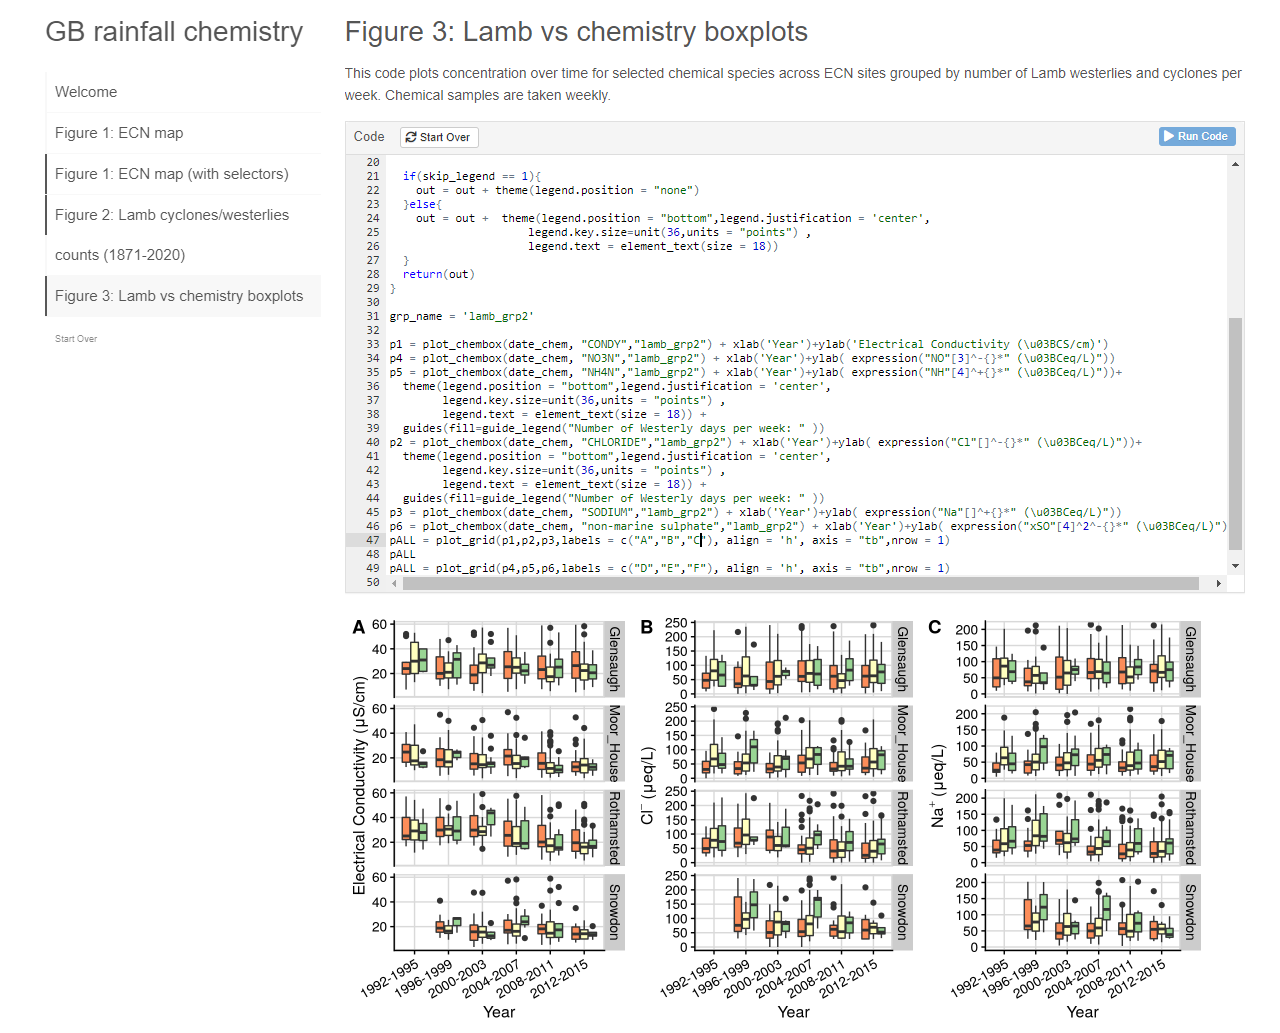
\includegraphics[width=\textwidth]{GB_notebook_screenshot} \caption[A screenshot of the GB rainfall interactive notebook site]{A screenshot of the GB rainfall interactive notebook site. The main feature is the code box. When the site loads, the code that generates published version of the figure is in the box and published version of the figure is below it. Users can make edits and re-run the code in the code box and the figure will update accordingly. Users can use the "Start Over" button to see the published version of the code at any point without refreshing the entire site.}\label{fig:fig2}
\end{figure}
\end{Schunk}

\hypertarget{evaluation}{%
\subsection{Evaluation}\label{evaluation}}

The main strength of our approach is that it fits nicely the gap of
existing approaches in terms of levels of abstraction. While code and
markdown documents gives full details of the code, standard Shiny apps
has too much limitations on users to interact with the code (Figure 3)
and users often cannot see the underlying code. Recently, it has become
popular to publish `live' Jupyter notebooks on Binder and Google Colab.
While this is a great contribution to open science, users are still
required to go run and go through the entire notebook step-by-step and
it can be easy to break it if users change something in between. Our
approach allows users to interact with portions of the code in a guided
and isolated manner, without the need to understand all the other parts
of a notebook or the fear to break it (Table 1). We emphasize that R
scripts/notebooks and R Shiny apps work well for their intended uses,
but our approach adds an additional level of accessibility to users.

The openness and ease-to-access our approach provides can benefit many
different stakeholders (Table 2). Researchers can more rapidly reproduce
\emph{parts} of the analysis of their choice without studying the entire
notebook or installing software or downloading all the data. They can
quickly test alternative hypothesis and stimulate scientific
discussions. For funders, encouraging the use of this approach means
less time is needed for future projects to pick up results from previous
work. And since this is based on \emph{learnr} which is originally
designed as a tutorial tool, this approach will no doubt speed up the
process to train other users to use similar methods. Overall, it
promotes open science and make a better value of public money.

An obvious limitation of our approach is that it does not work well for
ideal conditions where other R file formats are designed for. For
instance, R scripts and R notebooks are much better suited for more
complex analysis for users to adopt to their own problems. Meanwhile, R
Shiny provides a much richer user experience and is most suited when the
exposed code is generally not useful to stakeholders. Nevertheless, as
discussed above, our approach is designed for users to reproduce
\emph{elements} of an analysis. The user should evaluate these options
carefully, paying special attention to the needs of intended users.

\begin{Schunk}
\begin{figure}
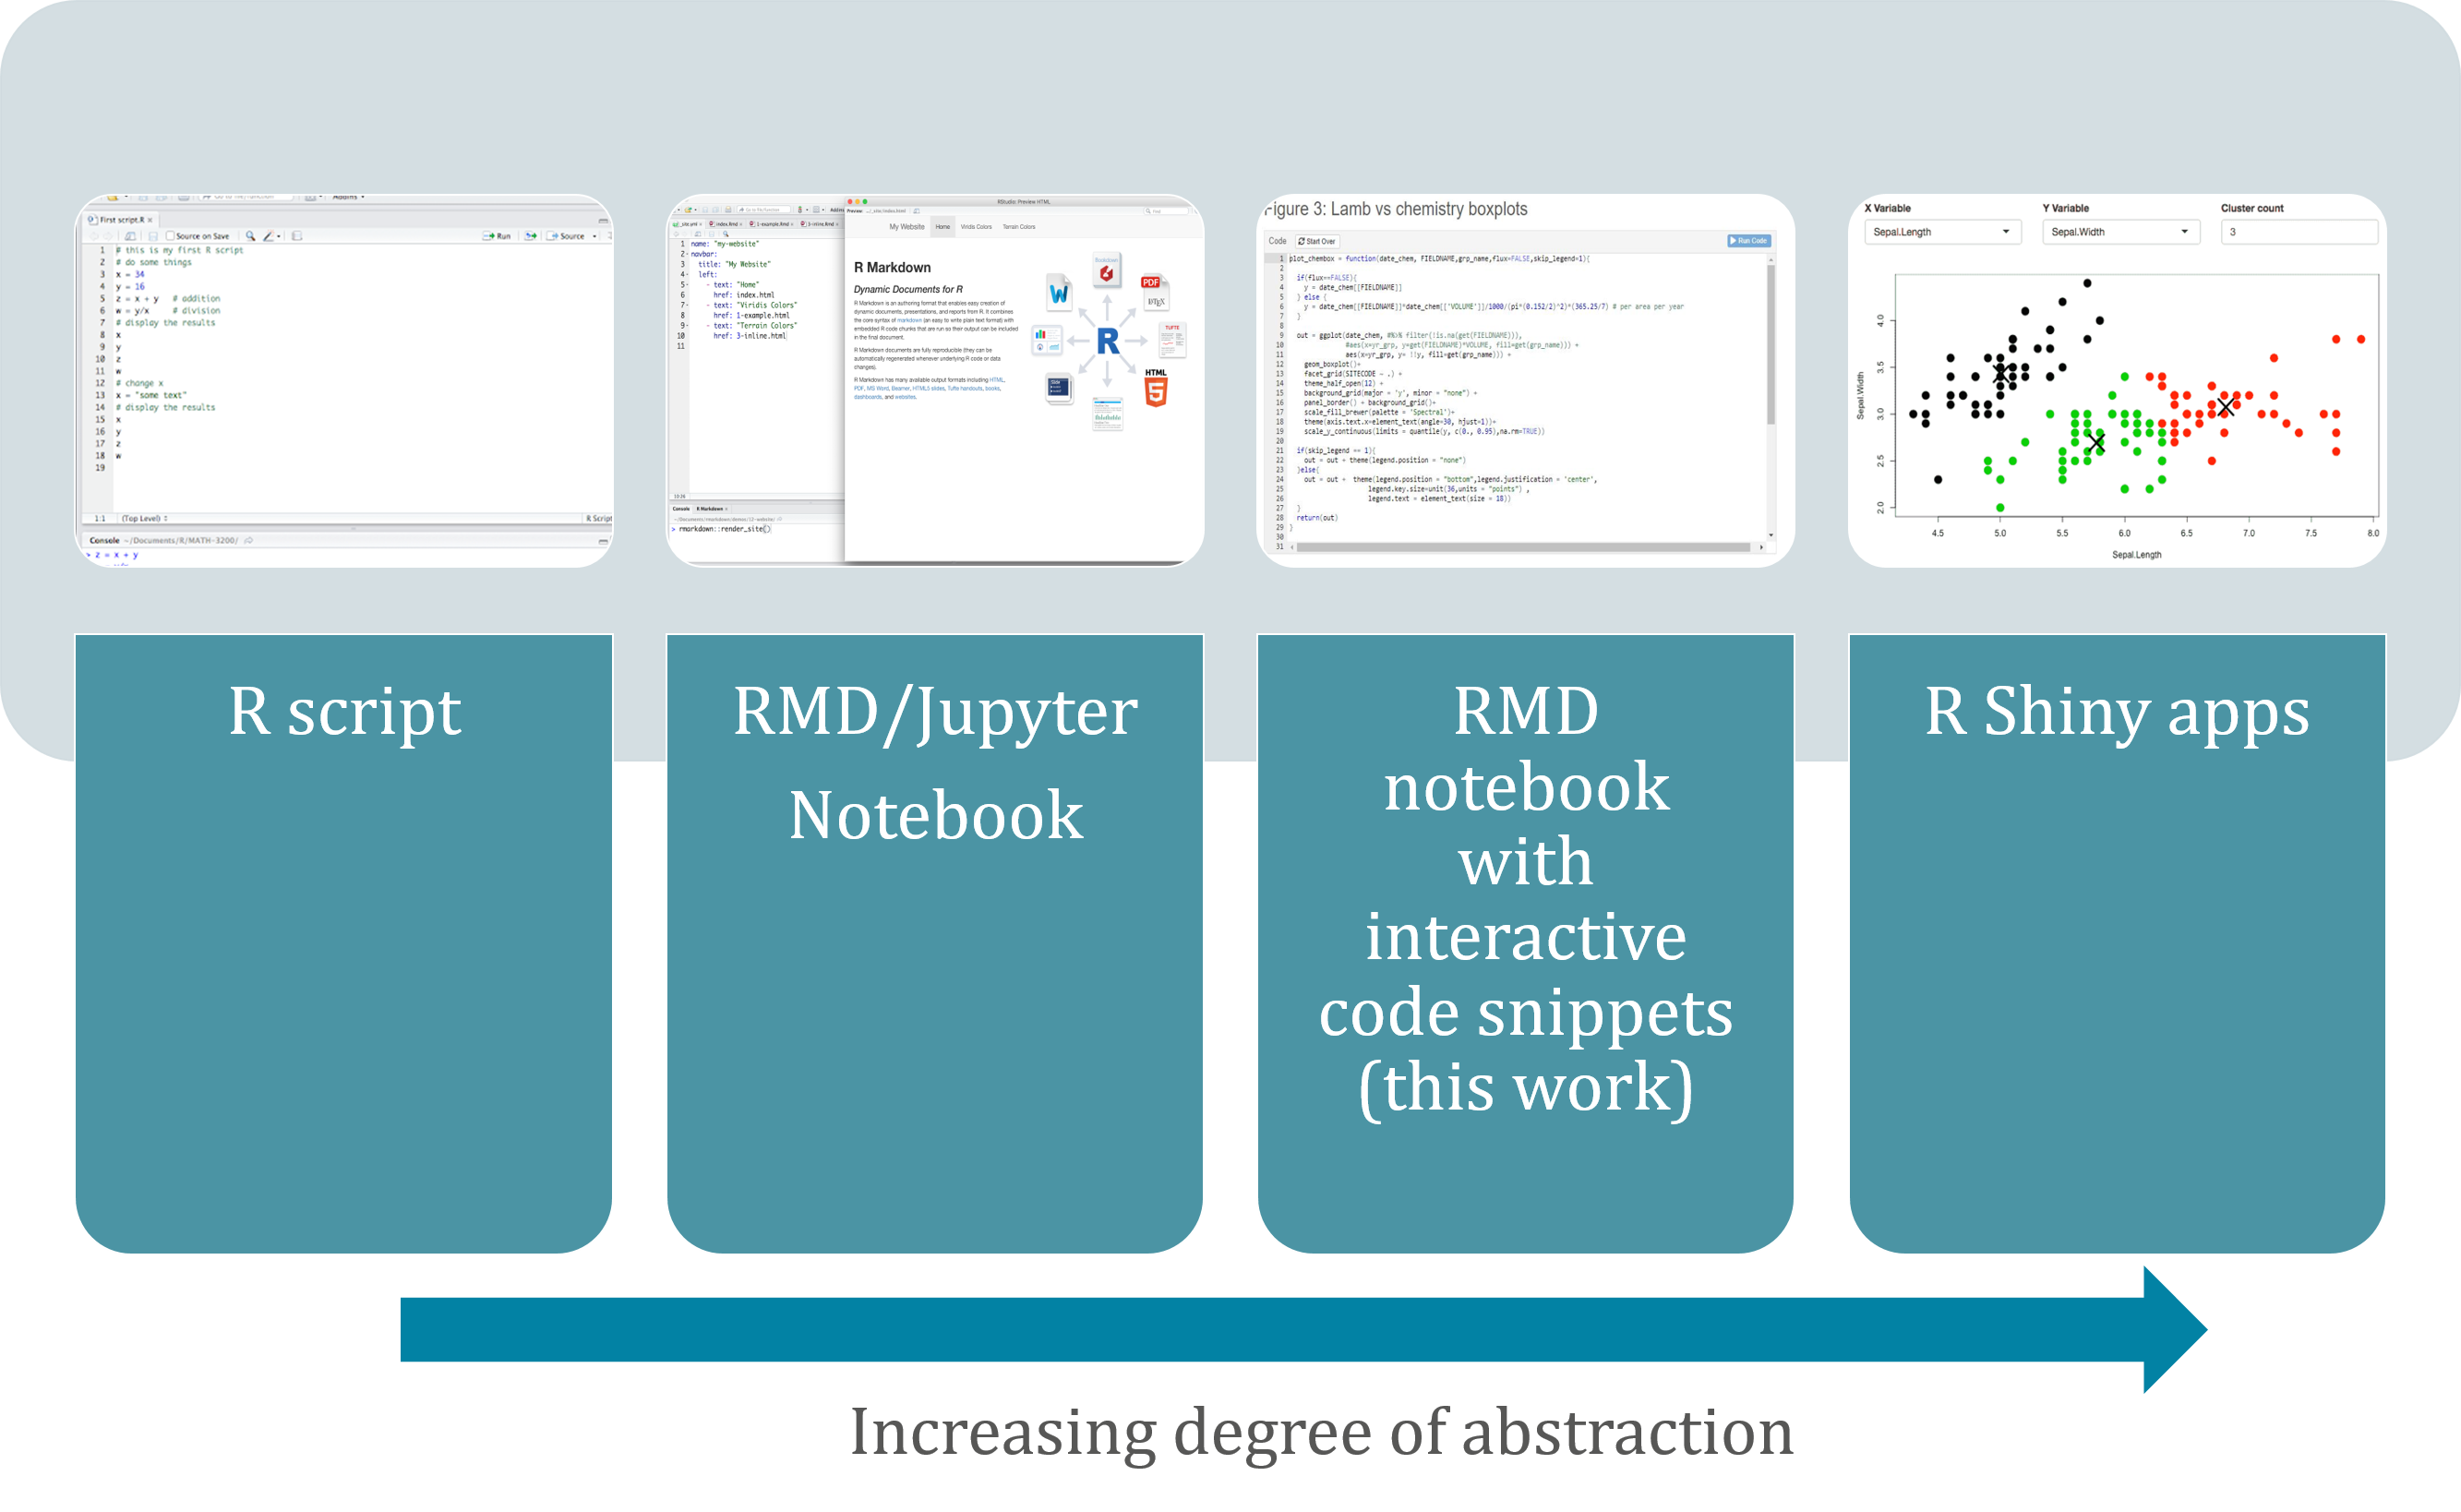
\includegraphics[width=\textwidth]{learnr_abstraction} \caption[The various levels of abstraction of various types of R documents]{The various levels of abstraction of various types of R documents. Our approach fills nicely the gap between R markdown or Jupyter notebooks and R Shiny apps.}\label{fig:fig1}
\end{figure}
\end{Schunk}

\begin{table}
  \caption{Advantages of the proposed approach over existing approaches}
  \label{tbl:table1}
  \includegraphics[width=\linewidth]{GB_notebook_table2}
\end{table}

\begin{table}
  \caption{Advantages of the proposed approach to various stakeholders}
  \label{tbl:table2}
  \includegraphics[width=\linewidth]{GB_notebook_table1}
\end{table}

Serving notebooks as a web service will inevitably face provenance
issues. It is surely beneficial if the author's institution can host
these interactive notebooks for a few years after its publication (and
that of its related publications). In the future, publishers and data
centres may consider providing services to provide longer term
provenance of serving these interactive notebooks online.

\hypertarget{summary-and-outlook}{%
\subsection{Summary and outlook}\label{summary-and-outlook}}

We have proposed and demonstrated a rapid approach to publish R markdown
notebooks as interactive sandboxes to allow users to experiment with
changes with various elements of a research output. It provides an
additional level of abstraction for users to interact with research
outputs and the codes that generates down. Since it can be linked to the
environment and data that generated the published output and has
independent document object identifiers (DOI), it is a suitable
candidate to preserve research workflow while exposing parts of it to
allow rapid experimentation by users. Our work is a demonstration on how
we may publish a notebook from virtual research environments such as
DataLabs, with data, packages, and workflow pre-loaded in a coding
envrionment, accompanied by rich narratives. While this paper outlines
the approach using R, the same approach can benefit other coding
languages such as Python. This can be achieved either through the
\emph{reticulate} (\citet{reticulate}) R package, or writing a python
package similar to \emph{learnr}. This paper contributes to the vision
towards publishing interactive notebooks as standalone research outputs
and the advancement of open science practices.

\hypertarget{data-availability}{%
\subsection{Data availability}\label{data-availability}}

The GB rainfall example notebook is accessible via this URL
(\url{https://cptecn-sandboxdemo.datalabs.ceh.ac.uk/}) and the R
markdown file is included as supplementary information. The DataLab code
stack is available at \url{https://github.com/NERC-CEH/datalab}. We
thank the DataLabs developers team (especially Iain Walmsley, UKCEH) for
the assitance to deploy interactive Rmd documents on DataLabs.

\bibliography{sandbox.bib}

\address{%
Chak Hau Michael Tso\\
UK Centre for Ecology and Hydrology\\%
Lancaster Environment Centre\\ Lancaster LA1 4YQ, United Kingdom\\
%
%
\\\textit{ORCiD: \href{https://orcid.org/0000-0002-2415-0826}{0000-0002-2415-0826}}%
\\\href{mailto:mtso@ceh.ac.uk}{\nolinkurl{mtso@ceh.ac.uk}}
}

\address{%
Michael Hollaway\\
UK Centre for Ecology and Hydrology\\%
Lancaster Environment Centre\\ Lancaster LA1 4YQ, United Kingdom\\
%
%
\\\textit{ORCiD: \href{https://orcid.org/0000-0003-0386-2696}{0000-0003-0386-2696}}%
\\\href{mailto:mhollaway@ceh.ac.uk}{\nolinkurl{mhollaway@ceh.ac.uk}}
}

\address{%
Rebecca Killick\\
Department of Statistics, Lancaster University\\%
Flyde College\\ Lancaster LA1 4YF, United Kingdom\\
%
%
\\\textit{ORCiD: \href{https://orcid.org/0000-0003-0583-3960}{0000-0003-0583-3960}}%
\\\href{mailto:r.killick@lancaster.ac.uk}{\nolinkurl{r.killick@lancaster.ac.uk}}
}

\address{%
Peter Henrys\\
UK Centre for Ecology and Hydrology\\%
Lancaster Environment Centre\\ Lancaster LA1 4YQ, United Kingdom\\
%
%
\\\textit{ORCiD: \href{https://orcid.org/0000-0003-4758-1482}{0000-0003-4758-1482}}%
\\\href{mailto:pehn@ceh.ac.uk}{\nolinkurl{pehn@ceh.ac.uk}}
}

\address{%
Don Monteith\\
UK Centre for Ecology and Hydrology\\%
Lancaster Environment Centre\\ Lancaster LA1 4YQ, United Kingdom\\
%
%
%
\\\href{mailto:donm@ceh.ac.uk}{\nolinkurl{donm@ceh.ac.uk}}
}

\address{%
John Watkins\\
UK Centre for Ecology and Hydrology\\%
Lancaster Environment Centre\\ Lancaster LA1 4YQ, United Kingdom\\
%
%
\\\textit{ORCiD: \href{https://orcid.org/0000-0002-3518-8918}{0000-0002-3518-8918}}%
\\\href{mailto:jww@ceh.ac.uk}{\nolinkurl{jww@ceh.ac.uk}}
}

\address{%
Gordon Blair\\
School of Computing and Communications, Lancaster University\\%
InfoLab21\\ Lancaster LA1 4WA, United Kingdom\\
%
%
\\\textit{ORCiD: \href{https://orcid.org/0000-0001-6212-1906}{0000-0001-6212-1906}}%
\\\href{mailto:g.blair@lancaster.ac.uk}{\nolinkurl{g.blair@lancaster.ac.uk}}
}

